% 散度 散度定理
% 多元微积分|矢量场|全微分|曲面积分|散度|divergence|源密度|source density|线性算符|散度定理

\pentry{全微分\upref{TDiff},曲面积分\upref{SurInt}, 流密度,}%未完成
我们在矢量场中取一个闭合曲面 $\mathcal{S}$,其内部空间记为 $\mathcal{V}$. 以向外为正方向,矢量场 $\bvec F(\bvec r)$ 在闭合曲面的通量 $\Phi$ 可以用以下面积分表示,积分范围默认为 $\mathcal{S}$
\begin{equation}\label{Divgnc_eq1}
\Phi  = \oint \bvec F \vdot \dd{\bvec a}
\end{equation}

现在我们把该曲面以其内部一点 $\bvec r$ 为中心按比例不断缩小,若通量与体积 $V$ 的比值存在极限,就把该极限叫做该点的\textbf{散度(divergence)},用 $\div$ 算符\footnote{符号 $\bvec\nabla$ 的名字为 nabla,作为算符时读作 del,一些教材也会在上方加矢量箭头,原因见下文.}记为(下文将介绍)
\begin{equation}\label{Divgnc_eq2}
\div \bvec F(\bvec r) \equiv \lim_{V \to 0} \frac{\Phi }{V}
\end{equation}
若场的分布连续且光滑,则该极限处处存在且与曲面的形状无关\footnote{本书不作证明},我们就得到了矢量场的散度场(注意是标量场).

\begin{example}{匀速水流}\label{Divgnc_ex1}
假设密度不变的水以匀速流动,质量的流密度场 $\bvec j(\bvec r)$ 为恒定场.对于任何一个闭合曲面,流入的流量(负值)和流出的流量(正值)相等,总通量为零. 所以该场的散度处处为零.
\end{example}

\begin{example}{变速水流}
在\autoref{Divgnc_ex1} 中,流密度场随 $x$ 坐标线性增加, $\bvec j = (j_0 + \alpha x)\uvec x$($\alpha$ 为常数),那么取一个边长为 $h$ 的立方体表面作为闭合曲面,从左侧的流量为 $\Phi_L =  - (j_0 + \alpha x_0) h^2$,右侧的流量为 $\Phi_R = [j_0 + \alpha (x_0 + h)] h^2$,其余四个面与 $\bvec j$ 平行,没有流量.闭合曲面的总流量为 $\Phi  = \alpha h^3 = \alpha V$. 根据定义,水流的散度处处为 $\alpha$. 分析可发现该水流中单位体积单位时间必然会凭空产生质量为 $\alpha$ 的水(虽然实际中不可能).所以散度也叫\textbf{源密度(source density)}.
\end{example}

\subsection{直角坐标系中的散度}

若在直角坐标系中给出矢量场
\begin{equation}
\bvec F(x,y,z) = F_x(x,y,z)\uvec x + F_y(x,y,z)\uvec y + F_z(x,y,z)\uvec z
\end{equation}
令闭合曲面为立方体 $[x,y,z]$-$[x+h,y+h,z+h]$ 的表面.先来考虑 $x$ 方向两个正方形的通量 $\Phi_x$,在点 $\bvec r (x,y,z)$ 附近对 $F_x(\bvec r)$ 使用全微分近似\upref{TDiff} 得(为简便书写,以下的函数值和偏导都默认在 $\bvec r$ 处取值)
\begin{equation}
F_x(x + x',y + y',z + z') \approx F_x + \pdv{F_x}{x}x' + \pdv{F_x}{y}y' + \pdv{F_x}{z}z'
\end{equation}
由于只有 $x$ 方向的场分量对 $\Phi_x$ 有贡献,
\begin{equation}
\ali{
\Phi_x &\approx \int_0^h \int_0^h \dd{y'}\dd{z'}  \cross \\
  &\phantom{\approx} \qty[ \qty( F_x + \pdv{F_x}{x}h + \pdv{F_x}{y}y' + \pdv{F_x}{z}z' ) - \qty( F_x + \pdv{F_x}{x}0 + \pdv{F_x}{y}y' + \pdv{F_x}{z}z' ) ] \\
   &= \pdv{F_x}{x}h \int_0^h \int_0^h \dd{y'}\dd{z'}  = \pdv{F_x}{x}h^3 = \pdv{F_x}{x}V
}\end{equation}
同理可以得到另外四个正方形的通量.六个正方形的总通量为
\begin{equation}
\Phi  \approx \qty( \pdv{F_x}{x} + \pdv{F_y}{y} + \pdv{F_z}{z} )V
\end{equation}
根据定义\autoref{Divgnc_eq2},可得直角坐标中的散度公式
\begin{equation}\label{Divgnc_eq7}
\div \bvec F = \lim_{V \to 0} \frac{\Phi }{V} = \pdv{F_x}{x} + \pdv{F_y}{y} + \pdv{F_z}{z}
\end{equation}
从形式上,我们可以引入一个 $\bvec\nabla$ 算符,在直角坐标系中的形式为
\begin{equation}
\bvec\nabla  = \uvec x\pdv{x} + \uvec y\pdv{y} + \uvec z\pdv{z}
\end{equation}
那么 $\div \bvec F(\bvec r)$ 从形式上可以看做矢量算符 $\bvec\nabla$ 与某点场矢量 $\bvec F(\bvec r)$ 的“内积”.根据\autoref{Divgnc_eq7},显然散度是一个\textbf{线性算符},即多个矢量场的线性组合的散度等于它们分别求散度再线性组合
\begin{equation}
\div [C_1 \bvec F_1(\bvec r) + C_2 \bvec F_2(\bvec r) + ...] = C_1 \div \bvec F_1(\bvec r) + C_2\div \bvec F_2(\bvec r) + \dots
\end{equation}

\begin{example}{质点引力场的散度}
令质点 $m$ 在坐标原点, 则它的引力场(\autoref{Gravty_eq2}~\upref{Gravty})为
\begin{equation}\label{Divgnc_eq10}
\bvec g(\bvec r) = -\frac{Gm}{r^3}\bvec r
\end{equation}
我们在直角坐标系中计算该场的散度. 直角坐标系中, 有 $\bvec r = x\uvec x + y\uvec y + z\uvec z$ 和 $r = \sqrt{x^2 + y^2 + z^2}$, 代入上式再求散度, 得
\begin{equation}\ali{
\div \bvec g &= \frac{Gm}{(x^2 + y^2 + z^2)^{5/2}} [(2x^2 - y^2 - z^2) + (2y^2 - z^2 - x^2) + (2z^2 - x^2 - y^2)]\\
&= 0
}\end{equation}
可见引力场的散度为 0. 然而需要注意的是, 在坐标原点处\autoref{Divgnc_eq10} 的各个方向的偏导都不存在, 所以不能用该公式计算散度. 以上的结论只适用于原点之外的点.
% 未完成:以后会在XXX详细讨论原点处的散度如何表示.
\end{example}

% 事实上, 该场在原点必定有无限大的散度, 如果作一个包含原点的高斯面, 其通量必为定值, 因为改变其形状, 散度的体积分并不改变(矢量场除了原点外散度处处为零)
% 未完成:另见柱坐标系中的散度,球坐标系中的散度,以及正交曲线坐标系中的散度

\subsection{散度定理}

我们来考虑一个有限大的闭合曲面并计算通量 $\Phi$. 我们先把曲面内的空间划分成许多体积足够小的微元,第 $i$ 个的体积微元为 $V_i$, 通量为 $\Phi_i \approx \div \bvec F(\bvec r_i) V_i$.现在来证明所有小曲面的通量之和等于大曲面的通量.
\begin{figure}[ht]
\centering
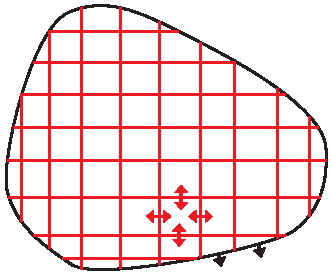
\includegraphics[width=5cm]{./figures/Divgnc_1.pdf}
\caption{证明所有小曲面的通量之和等于大曲面的通量} \label{Divgnc_fig1}
\end{figure}
\autoref{Divgnc_fig1} 中所有微元的曲面可划分为两部分,一是相邻两个小曲面的边界(红色),二是小曲面与大曲面重合的部分(黑色).前者产生的通量之和为零,因为这些边界都是由正方向相反的两块小曲面重合而成,它们产生的通量等大反向,互相抵消.后者产生的通量等于大曲面的通量,这是因为每块黑色边界都是由正方向相同的小曲面和大曲面重合而成,产生的通量等大同向.所以总通量等于
\begin{equation}
\Phi  = \sum_i \Phi_i  \approx \sum_i \div \bvec F (\bvec r_i) V_i
\end{equation}
令微元趋近无穷小,上面的求和变为定积分(积分范围默认为 $\mathcal V$ )
\begin{equation}\label{Divgnc_eq13}
\Phi  = \int \div \bvec F(\bvec r) \dd{V}
\end{equation}
所以\textbf{散度定理}就是,矢量场在任意闭合曲面的通量等于矢量场的散度在曲面所围空间的体积分.


% 未完成:例4 (给出一些场和曲面,证明散度定理成立)

